\documentclass{llncs}

\usepackage{graphicx}
\usepackage{placeins}

\begin{document}

\title{Dual MLP Pairs with Hidden Layer Sharing}

\author{Ivan Blagoev, Janeta Sevova, Kolyu Kolev}

% Ivan Blagoev i.blagoev@iit.bas.bg
% Janeta Sevova janetasevova@gmail.com
% Kolyu Kolev kolev_kolyu@yahoo.com

\institute{Institute of Information and Communication Technologies \\
Bulgarian Academy of Sciences \\
acad. Georgi Bonchev Str, block 2, office 514, 1113 Sofia, Bulgaria \\
\email{i.blagoev@iit.bas.bg} \\
\texttt{http://www.iict.bas.bg/}}

%----------------------------------------------------------------------------------------
%   Title
%----------------------------------------------------------------------------------------

\maketitle

%----------------------------------------------------------------------------------------
%   Abstract
%----------------------------------------------------------------------------------------

\begin{abstract}

Artificial neural networks (ANN) are well known and widely used from decades. One of the most popular kinds in the multilayer perceptron (MLP). Its general characteristic is that it has more than one layer. The most used topology of MLP has three layers (input, hidden and output). Layers are fully-connected between each other (the input with the hidden and the hidden with the output). The general disadvantage of this topology is that it does not has recurrent connections. Also the common usage of MLP is for single task solving. This research addresses these two common features of the MLP. Two MLPs are modified in such way that they share common hidden layer. Both MPLs have the task to forecast currency values (EUR/USD for the first one and USD/JPY for the second one). The lack of recurrent connections is solved by pairing each of the MLPs with another two MPLs. Pairs are done in such way that the output of the single MPL is take as input for its pairing MPL and the output of the pairing MPL is supplied at the original input. By such structure of four MPLs knowledge transfer is achieved by the shared hidden layer and short term memory is presented by the pairs. 

\keywords{artificial neural networks, multilayer perceptron, topologies}
\end{abstract}

%----------------------------------------------------------------------------------------
%   Paper
%----------------------------------------------------------------------------------------

\section{Introduction} \label{Introduction}

A general description of classical ANN is weighted directed graph. Networks usually consists of neurons and connections between them. The way in which neurons are connected between each other is called topology of the network. There are many topologies, but MLP is one of the most popular. As its name implies, MLP consists of layers. Many layers can be used in MLP, but the simplest variant is with three layers. Neurons in a neighbouring layers are fully connected usually. It means that each neuron in one layer has connections to all neurons of the neighbouring layer. The neurons in the input layer are connected with the external for the ANN world. In a similar way the output neurons are connected with the external for the ANN world. In the classical MLP networks the information goes from the input to the output. Such networks does not have feedback connections. Sometimes information can travel backward depending of the training algorithm. Such case is backpropagation training where ANN total error is distributed backward in order ANN weights to be adjusted. If MLP is accepted as monolite base more advanced topologies can be created. In this study MLPs sharing of the hidden layer is proposed. Such hidden layer sharing allows knowledge transfer between MPLs. Pairing of MLPs is also proposed in such way in which recurrent connections to be used and effect of ANN memory to be achieved. The proposed topology is very proper for big data analysis of time series \cite{atanasova01}. The paper is organized as follows: Section \ref{Introduction} introduces the problem; Section \ref{Topology Proposition} presents an ANN topology proposition; Section \ref{Experiments} gives some experiment details; Section \ref{Conclusions} concludes and some further ideas for research are pointed.

\section{Topology Proposition} \label{Topology Proposition}

A common disadvantage of the classical MLP is that it has no backward links. Due to the lack of such links there is no short term memory presented in such ANN topology. 

\begin{figure}
  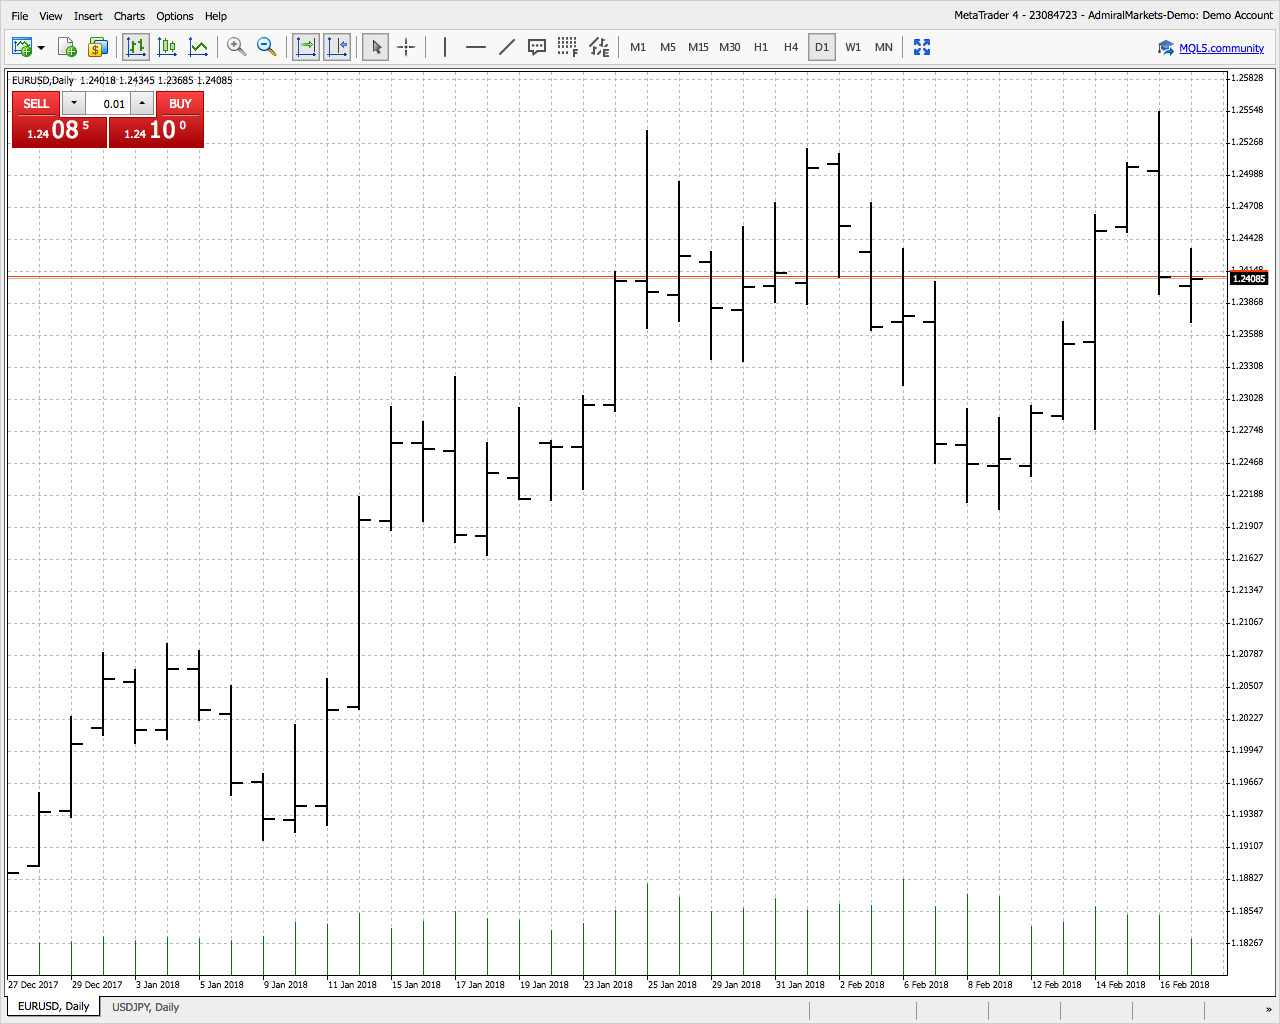
\includegraphics[width=1.0\linewidth]{fig01}
  \caption{MLP pairs with hidden layer sharing.}
  \label{fig01}
\end{figure}
\FloatBarrier

If simple MLP are taken as building blocks of a more complex ANN a variation of short term memory can be implemented (Fig. \ref{fig01}). The model proposed in this study uses four simple MLPs. The hidden layers of the two major MPLs are merged in a bigger shared layer. Such modification of the topology gives a way in which the information from the left MPL to travel in the right MPL and vice versa. Two other supportive MPLs are connected at the output of the major MPLs. The task of the supportive MPLs is to return some part of the signal at the input of the ANN structure. The output of the supportive MPLs is supplied at the shared hidden layer. As expected values on the supportive MPLs the input for major MPLs is used. 

\section{Experiments} \label{Experiments}

The experiments are done with Encog Neural Networks Framework for Java.

\begin{figure}
  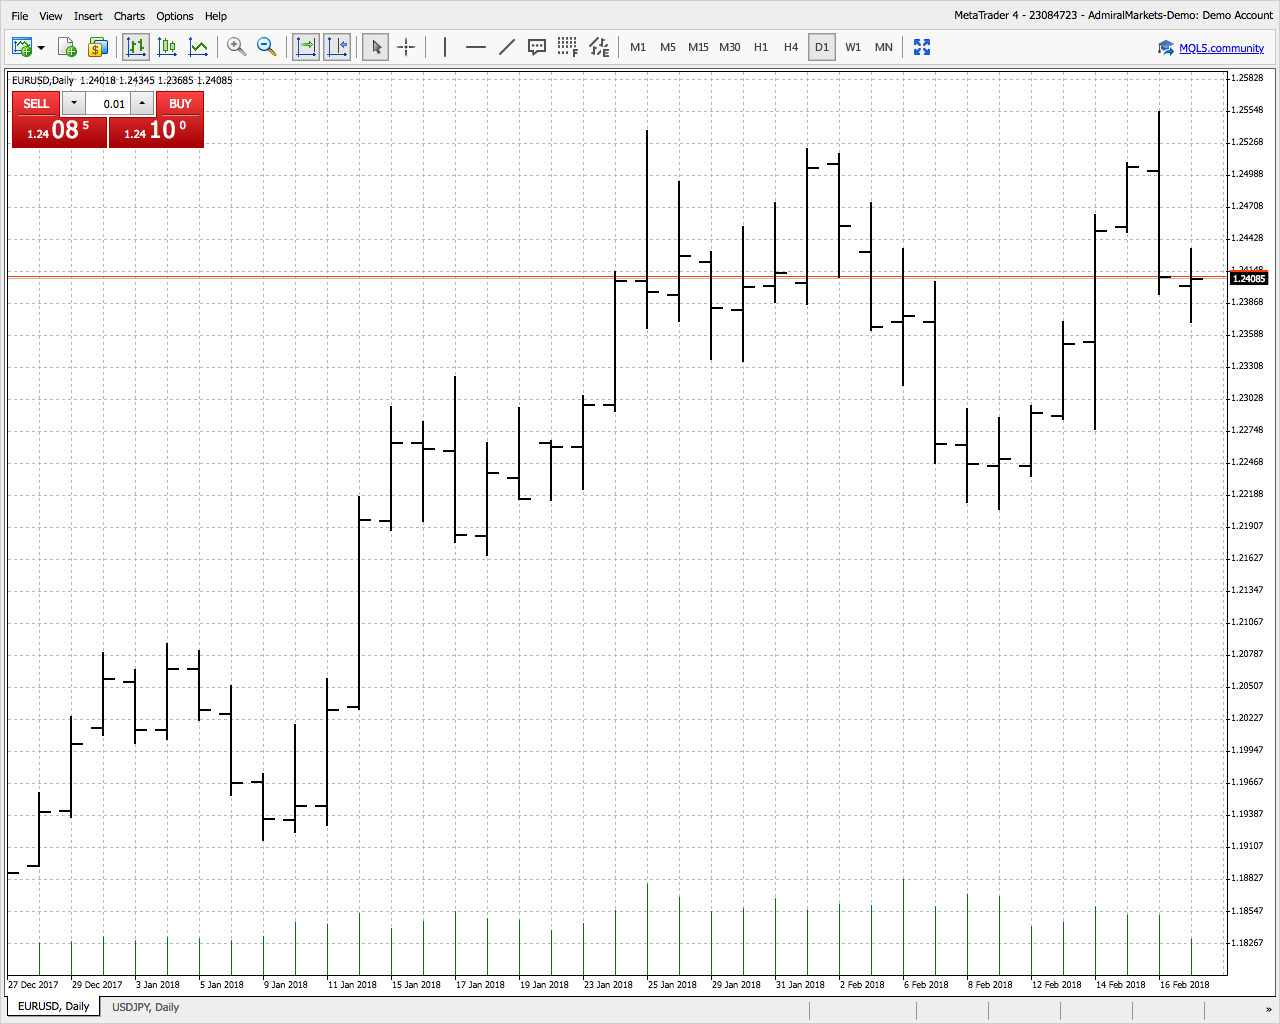
\includegraphics[width=1.0\linewidth]{fig02}
  \caption{Currencies values for two months on daily basis - EUR/USD currency pair.}
  \label{fig02}
\end{figure}
\FloatBarrier

As input data currencies values are used. One half of the ANN is supplied with EUR/USD values (Fig. \ref{fig02}). The other half of the ANN is supplied with USD/JPY values (Fig. \ref{fig03}). All data are normalized according the activation function levels. Data are separated in three sets: training (75\%), testing (20\%) and validation (25\%).  Validation set appears to be the most important part of the training, because according it the forecasting capabilities of the ANN are evaluated.

It is clearly visible (Fig. \ref{fig02} and Fig. \ref{fig03}) that the US economy is very related with the EU and Japanese economies. From forecasting point of view it is interesting that the correlation between both charts is negative. When EUR graph goes up the JPY graph goes down. It is something which ANN should learn and use effectively in the shared hidden layer. 

\begin{figure}
  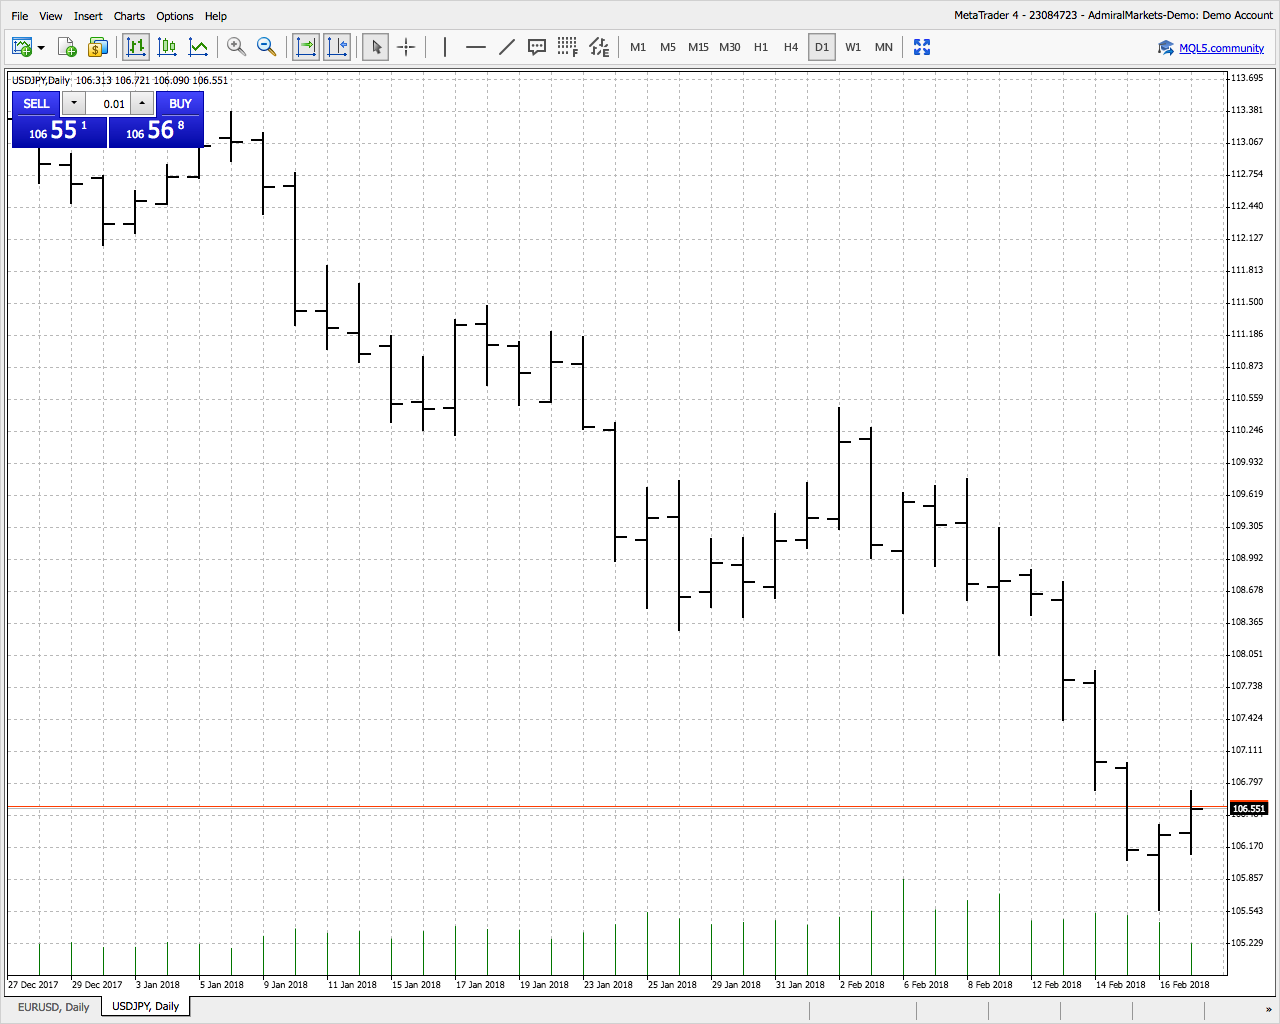
\includegraphics[width=1.0\linewidth]{fig03}
  \caption{Currencies values for two months on daily basis - USD/JPY currency pair.}
  \label{fig03}
\end{figure}
\FloatBarrier

\section{Conclusions} \label{Conclusions}

MLP based topologies can be very promising for financial time series forecasting. As further research this approach can be combined with Kalman Filter \cite{alexandrov01} or Generalized Nets \cite{tashev01,tashev02}. The effectiveness of the hidden layer sharing can be improved by permutation of the neurons as it is described in \cite{zankinski02}. ANN training in a distributed computing, as described in \cite{balabanov01,balabanov02,balabanov03,balabanov04,keremedchiev01,tomov01}, is also an interesting direction of further research. MLP neurons activation function is another direction of further research, as described in \cite{zankinski01}.

%----------------------------------------------------------------------------------------
%   Acknowledgements
%----------------------------------------------------------------------------------------

\section*{Acknowledgements}

This work was supported by private funding of Velbazhd Software LLC.

%----------------------------------------------------------------------------------------
%   Bibliography
%----------------------------------------------------------------------------------------

\begin{thebibliography}{99}

\bibitem{alexandrov01} Alexandrov, A., \textit{AD HOC Kalman filter based fusion algorithm for real-time Wireless Sensor Data Integration}, Proceedings of he Eleventh International Conference Flexible Quering Answering Systems, ISBN 978-3-319-26153-9, 151--160, Warsaw, Poland, 2015

\bibitem{atanasova01} Atanasova, T., Barova, M., Balabanov, T., \textit{Use of Neural Models for Analysis of Time Series in Big Data}, Publishing complex of "Vasil Levski" National Military University, ISSN 1314-1937, 193--198, 2016.

\bibitem{balabanov01} Balabanov, T., Genova, K., \textit{Distributed System for Artificial Neural Networks Training Based on Mobile Devices}, Proceedings of the International Conference Automatics and Informatics, Sofia, Bulgaria, Federation of the Scientific Engineering Unions John Atanasoff Society of Automatics and Informatics, ISSN 1313-1850, 49--52, 2016.

\bibitem{balabanov02} Balabanov, T., Keremedchiev, D., Goranov, I., \textit{Web Distributed Computing for Evolutionary Training of Artificial Neural Networks}, International Conference InfoTech, Varna - St. St. Constantine and Elena resort, Bulgaria, Publishing House of Technical University - Sofia, ISSN 1314-1023, 210--216, 2016.

\bibitem{balabanov03} Balabanov, T., Zankinski, I., Barova, M., \textit{Strategy for Individuals Distribution by Incident Nodes Participation in Star Topology of Distributed Evolutionary Algorithms}, Cybernetics and Information Technologies, Institute of Information and Communication Technologies - BAS, vol. 16, no. 1, ISSN 1311-9702, 80--88, 2016.

\bibitem{balabanov04} Balabanov, T., Zankinski, I., Dobrinkova, N., \textit{Time Series Prediction by Artificial Neural Networks and Differential Evolution in Distributed Environment}. Proceedings of the International Conference on Large-Scale Scientific Computing, Sozopol, Bulgaria, Lecture Notes in Computer Science, Springer, vol. 7116, no. 1, ISBN 978-3-642-29842-4, 198–205, 2011. 

\bibitem{keremedchiev01} Keremedchiev, D., Barova, M., Tomov, P., \textit{Mobile Application as Distributed Computing System for Artificial Neural Networks Training Used in Perfect Information Games}, Proceedings of the International Scientific Conference, UNITECH’16, Gabrovo, Bulgaria, ISSN 1313-230X, 389--393, 2016.

\bibitem{tashev01} Tashev, T., Marinov, M., Monov, V., Tasheva, R., \textit{Modeling of the MiMa-algorithm for crossbar switch by means of Generalized Nets}, Proceedings of the 2016 IEEE 8th International Conference on Intelligent Systems (IS), Sofia, Bulgaria, ISBN 978-1-5090-1354-8, 593--598, 2016.

\bibitem{tashev02} Tashev, T., Monov, V., \textit{Modeling of the hotspot load traffic for crossbar switch node by means of generalized nets}, Proceedings of the 6-th International IEEE Conference Intelligent Systems IS'12, Sofia, Bulgaria, vol. 2, 187--191, 2012.

\bibitem{tomov01} Tomov, P., Monov, V., \textit{Artificial Neural Networks and Differential Evolution Used for Time Series Forecasting in Distributed Environment}, Proceedings of the International Conference Automatics and Informatics, Sofia, Bulgaria, ISSN 1313-1850, 129--132, 2016.

\bibitem{zankinski01} Zankinski, I., Tomov, P., Balabanov, T., \textit{Alternative Activation Function Derivative in Artificial Neural Networks}, 25th Symposium with International Participation - Control of Energy, Industrial and Ecological Systems, Bankia, Bulgaria, John Atanasoff Union of Automation and Informatics, ISSN 1313-2237, 79--81, 2017.

\bibitem{zankinski02} Zankinski, I., Stoilov, T., \textit{Effect of the Neuron Permutation Problem on Training Artificial Neural Networks with Genetic Algorithms in Distributed Computing}, Proceedings of the 24th International Symposium Management of Energy, Industrial and Environmental Systems, ISSN 1313-2237, Bankya, Bulgaria, 53--55, 2016.

\end{thebibliography}

\end{document}
